\chapter{p3 = 20 (19 graphs)}
\newpage\begin{figure}
  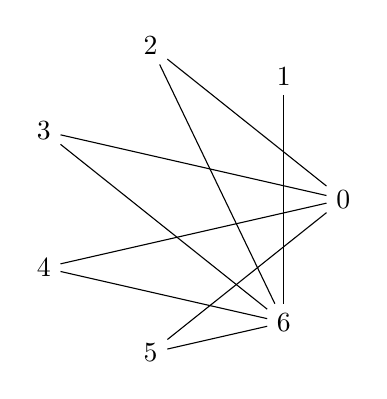
\begin{tikzpicture}
      \draw
        (0.0:2) node (0){0}
        (51.429:2) node (1){1}
        (102.857:2) node (2){2}
        (154.286:2) node (3){3}
        (205.714:2) node (4){4}
        (257.143:2) node (5){5}
        (308.571:2) node (6){6};
      \begin{scope}[-]
        \draw (0) to (2);
        \draw (0) to (3);
        \draw (0) to (4);
        \draw (0) to (5);
        \draw (1) to (6);
        \draw (2) to (6);
        \draw (3) to (6);
        \draw (4) to (6);
        \draw (5) to (6);
      \end{scope}
    \end{tikzpicture}
\end{figure}
\begin{itemize}
\item signature: 011110000010001001011
\item g: Graph with 7 nodes and 9 edges
\item order: 7
\item size: 9
\item max degree: 5
\item degrees: 1,2,2,2,2,4,5
\item is tree: 0
\item is bipartite: 1
\item has bridge: 1
\item is chordal: 0
\item is complete: 0
\item min cycle basis weight: 12
\item min cycle basis size: 3
\item diameter: 3
\item radius: 2
\item is eulerian: 0
\item is planar: 1
\item number of faces: 4
\item is regular: 0
\item p3: 20
\item p4: 4
\item property hash: d54dad0348dbaf64d40bfe85f687a035d16d8545ca422df558a739d41b0f7938
\end{itemize}
\newpage
\begin{figure}
  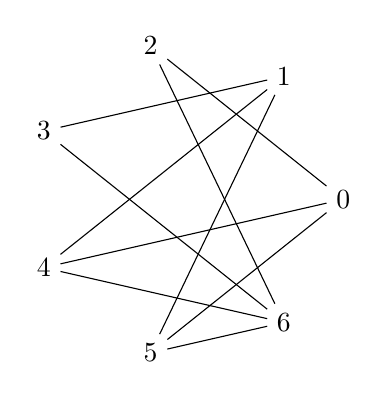
\begin{tikzpicture}
      \draw
        (0.0:2) node (0){0}
        (51.429:2) node (1){1}
        (102.857:2) node (2){2}
        (154.286:2) node (3){3}
        (205.714:2) node (4){4}
        (257.143:2) node (5){5}
        (308.571:2) node (6){6};
      \begin{scope}[-]
        \draw (0) to (2);
        \draw (0) to (4);
        \draw (0) to (5);
        \draw (1) to (3);
        \draw (1) to (4);
        \draw (1) to (5);
        \draw (2) to (6);
        \draw (3) to (6);
        \draw (4) to (6);
        \draw (5) to (6);
      \end{scope}
    \end{tikzpicture}
\end{figure}
\begin{itemize}
\item signature: 010110011100001001011
\item g: Graph with 7 nodes and 10 edges
\item order: 7
\item size: 10
\item max degree: 4
\item degrees: 2,2,3,3,3,3,4
\item is tree: 0
\item is bipartite: 1
\item has bridge: 0
\item is chordal: 0
\item is complete: 0
\item min cycle basis weight: 16
\item min cycle basis size: 4
\item diameter: 3
\item radius: 2
\item is eulerian: 0
\item is planar: 1
\item number of faces: 5
\item is regular: 0
\item p3: 20
\item p4: 10
\item property hash: 4699f61cf5c8d538d0c5f03d06ba4c67737a27be99410f2a6b548312da52b889
\end{itemize}
\newpage
\begin{figure}
  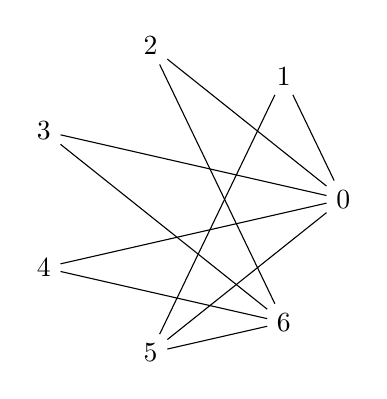
\begin{tikzpicture}
      \draw
        (0.0:2) node (0){0}
        (51.429:2) node (1){1}
        (102.857:2) node (2){2}
        (154.286:2) node (3){3}
        (205.714:2) node (4){4}
        (257.143:2) node (5){5}
        (308.571:2) node (6){6};
      \begin{scope}[-]
        \draw (0) to (1);
        \draw (0) to (2);
        \draw (0) to (3);
        \draw (0) to (4);
        \draw (0) to (5);
        \draw (1) to (5);
        \draw (2) to (6);
        \draw (3) to (6);
        \draw (4) to (6);
        \draw (5) to (6);
      \end{scope}
    \end{tikzpicture}
\end{figure}
\begin{itemize}
\item signature: 111110000100001001011
\item g: Graph with 7 nodes and 10 edges
\item order: 7
\item size: 10
\item max degree: 5
\item degrees: 2,2,2,2,3,4,5
\item is tree: 0
\item is bipartite: 0
\item has bridge: 0
\item is chordal: 0
\item is complete: 0
\item min cycle basis weight: 15
\item min cycle basis size: 4
\item diameter: 2
\item radius: 2
\item is eulerian: 0
\item is planar: 1
\item number of faces: 5
\item is regular: 0
\item p3: 20
\item p4: None
\item property hash: 29c6d4d1d8aea4097135462206ad0a5d84b950e5dd939cb53d2c2cc3d140ac0a
\end{itemize}
\newpage
\begin{figure}
  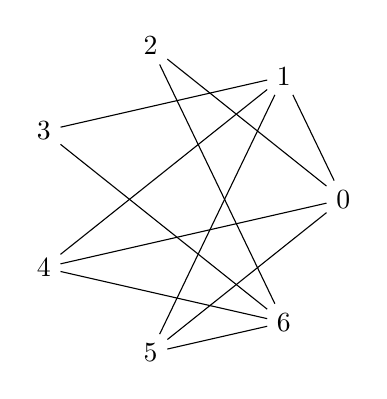
\begin{tikzpicture}
      \draw
        (0.0:2) node (0){0}
        (51.429:2) node (1){1}
        (102.857:2) node (2){2}
        (154.286:2) node (3){3}
        (205.714:2) node (4){4}
        (257.143:2) node (5){5}
        (308.571:2) node (6){6};
      \begin{scope}[-]
        \draw (0) to (1);
        \draw (0) to (2);
        \draw (0) to (4);
        \draw (0) to (5);
        \draw (1) to (3);
        \draw (1) to (4);
        \draw (1) to (5);
        \draw (2) to (6);
        \draw (3) to (6);
        \draw (4) to (6);
        \draw (5) to (6);
      \end{scope}
    \end{tikzpicture}
\end{figure}
\begin{itemize}
\item signature: 110110011100001001011
\item g: Graph with 7 nodes and 11 edges
\item order: 7
\item size: 11
\item max degree: 4
\item degrees: 2,2,3,3,4,4,4
\item is tree: 0
\item is bipartite: 0
\item has bridge: 0
\item is chordal: 0
\item is complete: 0
\item min cycle basis weight: 18
\item min cycle basis size: 5
\item diameter: 2
\item radius: 2
\item is eulerian: 0
\item is planar: 1
\item number of faces: 6
\item is regular: 0
\item p3: 20
\item p4: 9
\item property hash: eec644903c903b67f82a355a0d11b0615df2af4388cd8f90eb3fb3ec3f000c9f
\end{itemize}
\newpage
\begin{figure}
  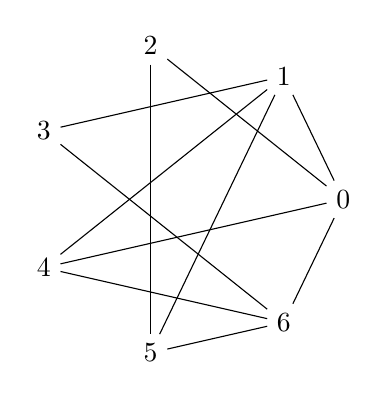
\begin{tikzpicture}
      \draw
        (0.0:2) node (0){0}
        (51.429:2) node (1){1}
        (102.857:2) node (2){2}
        (154.286:2) node (3){3}
        (205.714:2) node (4){4}
        (257.143:2) node (5){5}
        (308.571:2) node (6){6};
      \begin{scope}[-]
        \draw (0) to (1);
        \draw (0) to (2);
        \draw (0) to (4);
        \draw (0) to (6);
        \draw (1) to (3);
        \draw (1) to (4);
        \draw (1) to (5);
        \draw (2) to (5);
        \draw (3) to (6);
        \draw (4) to (6);
        \draw (5) to (6);
      \end{scope}
    \end{tikzpicture}
\end{figure}
\begin{itemize}
\item signature: 110101011100010001011
\item g: Graph with 7 nodes and 11 edges
\item order: 7
\item size: 11
\item max degree: 4
\item degrees: 2,2,3,3,4,4,4
\item is tree: 0
\item is bipartite: 0
\item has bridge: 0
\item is chordal: 0
\item is complete: 0
\item min cycle basis weight: 18
\item min cycle basis size: 5
\item diameter: 3
\item radius: 2
\item is eulerian: 0
\item is planar: 1
\item number of faces: 6
\item is regular: 0
\item p3: 20
\item p4: 7
\item property hash: 74c0d85707791c3321f2153702d0cc6b735370c018d84e3c17335d9754419d4c
\end{itemize}
\newpage
\begin{figure}
  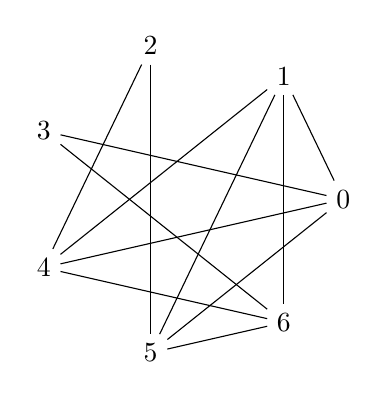
\begin{tikzpicture}
      \draw
        (0.0:2) node (0){0}
        (51.429:2) node (1){1}
        (102.857:2) node (2){2}
        (154.286:2) node (3){3}
        (205.714:2) node (4){4}
        (257.143:2) node (5){5}
        (308.571:2) node (6){6};
      \begin{scope}[-]
        \draw (0) to (1);
        \draw (0) to (3);
        \draw (0) to (4);
        \draw (0) to (5);
        \draw (1) to (4);
        \draw (1) to (5);
        \draw (1) to (6);
        \draw (2) to (4);
        \draw (2) to (5);
        \draw (3) to (6);
        \draw (4) to (6);
        \draw (5) to (6);
      \end{scope}
    \end{tikzpicture}
\end{figure}
\begin{itemize}
\item signature: 101110001110110001011
\item g: Graph with 7 nodes and 12 edges
\item order: 7
\item size: 12
\item max degree: 4
\item degrees: 2,2,4,4,4,4,4
\item is tree: 0
\item is bipartite: 0
\item has bridge: 0
\item is chordal: 0
\item is complete: 0
\item min cycle basis weight: 20
\item min cycle basis size: 6
\item diameter: 3
\item radius: 2
\item is eulerian: 1
\item is planar: 0
\item number of faces: 7
\item is regular: 0
\item p3: 20
\item p4: None
\item property hash: c734b01b25361c4592816338c04ff6c953908bbd334b681f60fc4360718232e4
\end{itemize}
\newpage
\begin{figure}
  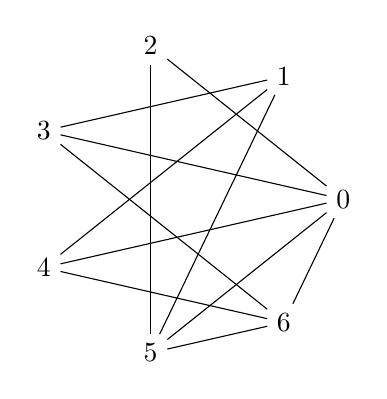
\begin{tikzpicture}
      \draw
        (0.0:2) node (0){0}
        (51.429:2) node (1){1}
        (102.857:2) node (2){2}
        (154.286:2) node (3){3}
        (205.714:2) node (4){4}
        (257.143:2) node (5){5}
        (308.571:2) node (6){6};
      \begin{scope}[-]
        \draw (0) to (2);
        \draw (0) to (3);
        \draw (0) to (4);
        \draw (0) to (5);
        \draw (0) to (6);
        \draw (1) to (3);
        \draw (1) to (4);
        \draw (1) to (5);
        \draw (2) to (5);
        \draw (3) to (6);
        \draw (4) to (6);
        \draw (5) to (6);
      \end{scope}
    \end{tikzpicture}
\end{figure}
\begin{itemize}
\item signature: 011111011100010001011
\item g: Graph with 7 nodes and 12 edges
\item order: 7
\item size: 12
\item max degree: 5
\item degrees: 2,3,3,3,4,4,5
\item is tree: 0
\item is bipartite: 0
\item has bridge: 0
\item is chordal: 0
\item is complete: 0
\item min cycle basis weight: 20
\item min cycle basis size: 6
\item diameter: 2
\item radius: 2
\item is eulerian: 0
\item is planar: 0
\item number of faces: 7
\item is regular: 0
\item p3: 20
\item p4: None
\item property hash: 36fcd8db5b066db761f05f8f70721e9058517aac227a61acd9535dc7bc832ce1
\end{itemize}
\newpage
\begin{figure}
  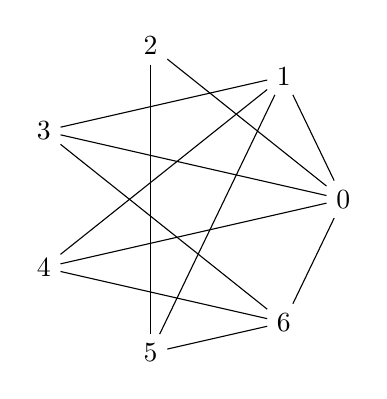
\begin{tikzpicture}
      \draw
        (0.0:2) node (0){0}
        (51.429:2) node (1){1}
        (102.857:2) node (2){2}
        (154.286:2) node (3){3}
        (205.714:2) node (4){4}
        (257.143:2) node (5){5}
        (308.571:2) node (6){6};
      \begin{scope}[-]
        \draw (0) to (1);
        \draw (0) to (2);
        \draw (0) to (3);
        \draw (0) to (4);
        \draw (0) to (6);
        \draw (1) to (3);
        \draw (1) to (4);
        \draw (1) to (5);
        \draw (2) to (5);
        \draw (3) to (6);
        \draw (4) to (6);
        \draw (5) to (6);
      \end{scope}
    \end{tikzpicture}
\end{figure}
\begin{itemize}
\item signature: 111101011100010001011
\item g: Graph with 7 nodes and 12 edges
\item order: 7
\item size: 12
\item max degree: 5
\item degrees: 2,3,3,3,4,4,5
\item is tree: 0
\item is bipartite: 0
\item has bridge: 0
\item is chordal: 0
\item is complete: 0
\item min cycle basis weight: 20
\item min cycle basis size: 6
\item diameter: 2
\item radius: 2
\item is eulerian: 0
\item is planar: 0
\item number of faces: 7
\item is regular: 0
\item p3: 20
\item p4: None
\item property hash: 36fcd8db5b066db761f05f8f70721e9058517aac227a61acd9535dc7bc832ce1
\end{itemize}
\newpage
\begin{figure}
  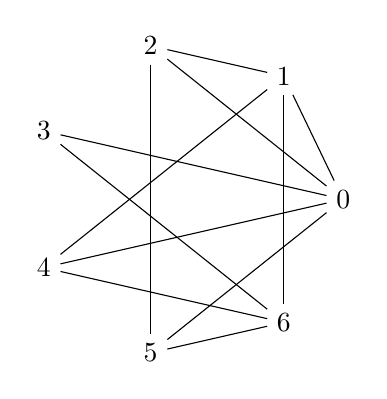
\begin{tikzpicture}
      \draw
        (0.0:2) node (0){0}
        (51.429:2) node (1){1}
        (102.857:2) node (2){2}
        (154.286:2) node (3){3}
        (205.714:2) node (4){4}
        (257.143:2) node (5){5}
        (308.571:2) node (6){6};
      \begin{scope}[-]
        \draw (0) to (1);
        \draw (0) to (2);
        \draw (0) to (3);
        \draw (0) to (4);
        \draw (0) to (5);
        \draw (1) to (2);
        \draw (1) to (4);
        \draw (1) to (6);
        \draw (2) to (5);
        \draw (3) to (6);
        \draw (4) to (6);
        \draw (5) to (6);
      \end{scope}
    \end{tikzpicture}
\end{figure}
\begin{itemize}
\item signature: 111110101010010001011
\item g: Graph with 7 nodes and 12 edges
\item order: 7
\item size: 12
\item max degree: 5
\item degrees: 2,3,3,3,4,4,5
\item is tree: 0
\item is bipartite: 0
\item has bridge: 0
\item is chordal: 0
\item is complete: 0
\item min cycle basis weight: 20
\item min cycle basis size: 6
\item diameter: 2
\item radius: 2
\item is eulerian: 0
\item is planar: 1
\item number of faces: 7
\item is regular: 0
\item p3: 20
\item p4: None
\item property hash: 7182713288bc30e43b0ae5236072a18f4fa32f9c8eaf9fb9c10f2a928640378f
\end{itemize}
\newpage
\begin{figure}
  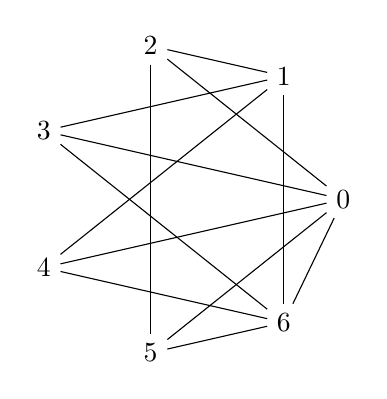
\begin{tikzpicture}
      \draw
        (0.0:2) node (0){0}
        (51.429:2) node (1){1}
        (102.857:2) node (2){2}
        (154.286:2) node (3){3}
        (205.714:2) node (4){4}
        (257.143:2) node (5){5}
        (308.571:2) node (6){6};
      \begin{scope}[-]
        \draw (0) to (2);
        \draw (0) to (3);
        \draw (0) to (4);
        \draw (0) to (5);
        \draw (0) to (6);
        \draw (1) to (2);
        \draw (1) to (3);
        \draw (1) to (4);
        \draw (1) to (6);
        \draw (2) to (5);
        \draw (3) to (6);
        \draw (4) to (6);
        \draw (5) to (6);
      \end{scope}
    \end{tikzpicture}
\end{figure}
\begin{itemize}
\item signature: 011111111010010001011
\item g: Graph with 7 nodes and 13 edges
\item order: 7
\item size: 13
\item max degree: 5
\item degrees: 3,3,3,3,4,5,5
\item is tree: 0
\item is bipartite: 0
\item has bridge: 0
\item is chordal: 0
\item is complete: 0
\item min cycle basis weight: 22
\item min cycle basis size: 7
\item diameter: 2
\item radius: 2
\item is eulerian: 0
\item is planar: 0
\item number of faces: 8
\item is regular: 0
\item p3: 20
\item p4: None
\item property hash: 9e8edb1c24e705dc57fbf9e6a026d65a005d6ede021b60db47414040f3e8824c
\end{itemize}
\newpage
\begin{figure}
  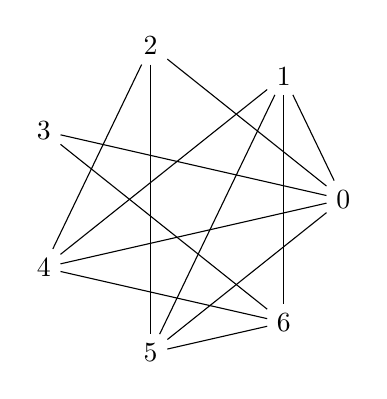
\begin{tikzpicture}
      \draw
        (0.0:2) node (0){0}
        (51.429:2) node (1){1}
        (102.857:2) node (2){2}
        (154.286:2) node (3){3}
        (205.714:2) node (4){4}
        (257.143:2) node (5){5}
        (308.571:2) node (6){6};
      \begin{scope}[-]
        \draw (0) to (1);
        \draw (0) to (2);
        \draw (0) to (3);
        \draw (0) to (4);
        \draw (0) to (5);
        \draw (1) to (4);
        \draw (1) to (5);
        \draw (1) to (6);
        \draw (2) to (4);
        \draw (2) to (5);
        \draw (3) to (6);
        \draw (4) to (6);
        \draw (5) to (6);
      \end{scope}
    \end{tikzpicture}
\end{figure}
\begin{itemize}
\item signature: 111110001110110001011
\item g: Graph with 7 nodes and 13 edges
\item order: 7
\item size: 13
\item max degree: 5
\item degrees: 2,3,4,4,4,4,5
\item is tree: 0
\item is bipartite: 0
\item has bridge: 0
\item is chordal: 0
\item is complete: 0
\item min cycle basis weight: 22
\item min cycle basis size: 7
\item diameter: 2
\item radius: 2
\item is eulerian: 0
\item is planar: 0
\item number of faces: 8
\item is regular: 0
\item p3: 20
\item p4: None
\item property hash: 266d7285b93bb41f10ade986c85aaa67e57051741038765db740895c8677ebd9
\end{itemize}
\newpage
\begin{figure}
  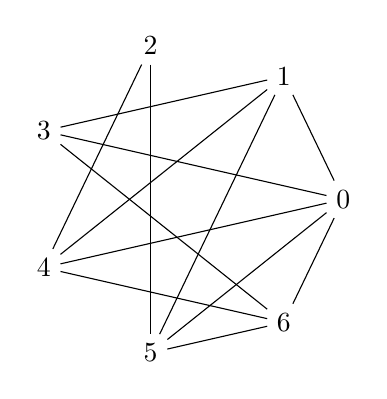
\begin{tikzpicture}
      \draw
        (0.0:2) node (0){0}
        (51.429:2) node (1){1}
        (102.857:2) node (2){2}
        (154.286:2) node (3){3}
        (205.714:2) node (4){4}
        (257.143:2) node (5){5}
        (308.571:2) node (6){6};
      \begin{scope}[-]
        \draw (0) to (1);
        \draw (0) to (3);
        \draw (0) to (4);
        \draw (0) to (5);
        \draw (0) to (6);
        \draw (1) to (3);
        \draw (1) to (4);
        \draw (1) to (5);
        \draw (2) to (4);
        \draw (2) to (5);
        \draw (3) to (6);
        \draw (4) to (6);
        \draw (5) to (6);
      \end{scope}
    \end{tikzpicture}
\end{figure}
\begin{itemize}
\item signature: 101111011100110001011
\item g: Graph with 7 nodes and 13 edges
\item order: 7
\item size: 13
\item max degree: 5
\item degrees: 2,3,4,4,4,4,5
\item is tree: 0
\item is bipartite: 0
\item has bridge: 0
\item is chordal: 0
\item is complete: 0
\item min cycle basis weight: 22
\item min cycle basis size: 7
\item diameter: 3
\item radius: 2
\item is eulerian: 0
\item is planar: 0
\item number of faces: 8
\item is regular: 0
\item p3: 20
\item p4: None
\item property hash: 971417b4a736c903e71c3e6ca29a0a0b08303de815c4032ec30b8e37439b0957
\end{itemize}
\newpage
\begin{figure}
  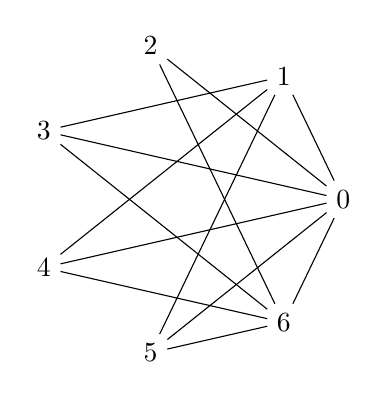
\begin{tikzpicture}
      \draw
        (0.0:2) node (0){0}
        (51.429:2) node (1){1}
        (102.857:2) node (2){2}
        (154.286:2) node (3){3}
        (205.714:2) node (4){4}
        (257.143:2) node (5){5}
        (308.571:2) node (6){6};
      \begin{scope}[-]
        \draw (0) to (1);
        \draw (0) to (2);
        \draw (0) to (3);
        \draw (0) to (4);
        \draw (0) to (5);
        \draw (0) to (6);
        \draw (1) to (3);
        \draw (1) to (4);
        \draw (1) to (5);
        \draw (2) to (6);
        \draw (3) to (6);
        \draw (4) to (6);
        \draw (5) to (6);
      \end{scope}
    \end{tikzpicture}
\end{figure}
\begin{itemize}
\item signature: 111111011100001001011
\item g: Graph with 7 nodes and 13 edges
\item order: 7
\item size: 13
\item max degree: 6
\item degrees: 2,3,3,3,4,5,6
\item is tree: 0
\item is bipartite: 0
\item has bridge: 0
\item is chordal: 0
\item is complete: 0
\item min cycle basis weight: 21
\item min cycle basis size: 7
\item diameter: 2
\item radius: 1
\item is eulerian: 0
\item is planar: 0
\item number of faces: 8
\item is regular: 0
\item p3: 20
\item p4: None
\item property hash: 4183e784f1fa6a5647e34847b0e308fac8e8896f1eec7f5f9daf0c659fa6d58f
\end{itemize}
\newpage
\begin{figure}
  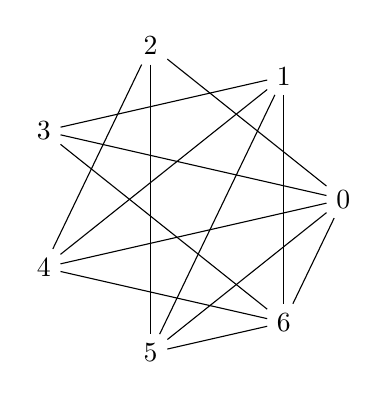
\begin{tikzpicture}
      \draw
        (0.0:2) node (0){0}
        (51.429:2) node (1){1}
        (102.857:2) node (2){2}
        (154.286:2) node (3){3}
        (205.714:2) node (4){4}
        (257.143:2) node (5){5}
        (308.571:2) node (6){6};
      \begin{scope}[-]
        \draw (0) to (2);
        \draw (0) to (3);
        \draw (0) to (4);
        \draw (0) to (5);
        \draw (0) to (6);
        \draw (1) to (3);
        \draw (1) to (4);
        \draw (1) to (5);
        \draw (1) to (6);
        \draw (2) to (4);
        \draw (2) to (5);
        \draw (3) to (6);
        \draw (4) to (6);
        \draw (5) to (6);
      \end{scope}
    \end{tikzpicture}
\end{figure}
\begin{itemize}
\item signature: 011111011110110001011
\item g: Graph with 7 nodes and 14 edges
\item order: 7
\item size: 14
\item max degree: 5
\item degrees: 3,3,4,4,4,5,5
\item is tree: 0
\item is bipartite: 0
\item has bridge: 0
\item is chordal: 0
\item is complete: 0
\item min cycle basis weight: 24
\item min cycle basis size: 8
\item diameter: 2
\item radius: 2
\item is eulerian: 0
\item is planar: 0
\item number of faces: 9
\item is regular: 0
\item p3: 20
\item p4: None
\item property hash: d647de3c90190efa45df7b9d806cc4b262fb825f5374192c7636ea2fc83f7864
\end{itemize}
\newpage
\begin{figure}
  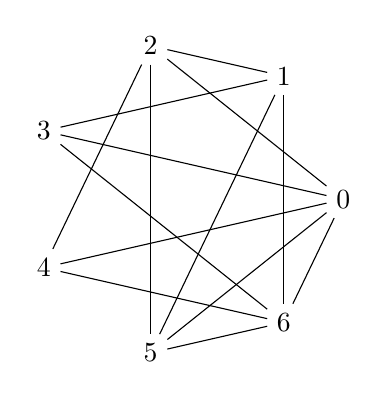
\begin{tikzpicture}
      \draw
        (0.0:2) node (0){0}
        (51.429:2) node (1){1}
        (102.857:2) node (2){2}
        (154.286:2) node (3){3}
        (205.714:2) node (4){4}
        (257.143:2) node (5){5}
        (308.571:2) node (6){6};
      \begin{scope}[-]
        \draw (0) to (2);
        \draw (0) to (3);
        \draw (0) to (4);
        \draw (0) to (5);
        \draw (0) to (6);
        \draw (1) to (2);
        \draw (1) to (3);
        \draw (1) to (5);
        \draw (1) to (6);
        \draw (2) to (4);
        \draw (2) to (5);
        \draw (3) to (6);
        \draw (4) to (6);
        \draw (5) to (6);
      \end{scope}
    \end{tikzpicture}
\end{figure}
\begin{itemize}
\item signature: 011111110110110001011
\item g: Graph with 7 nodes and 14 edges
\item order: 7
\item size: 14
\item max degree: 5
\item degrees: 3,3,4,4,4,5,5
\item is tree: 0
\item is bipartite: 0
\item has bridge: 0
\item is chordal: 0
\item is complete: 0
\item min cycle basis weight: 24
\item min cycle basis size: 8
\item diameter: 2
\item radius: 2
\item is eulerian: 0
\item is planar: 0
\item number of faces: 9
\item is regular: 0
\item p3: 20
\item p4: None
\item property hash: d647de3c90190efa45df7b9d806cc4b262fb825f5374192c7636ea2fc83f7864
\end{itemize}
\newpage
\begin{figure}
  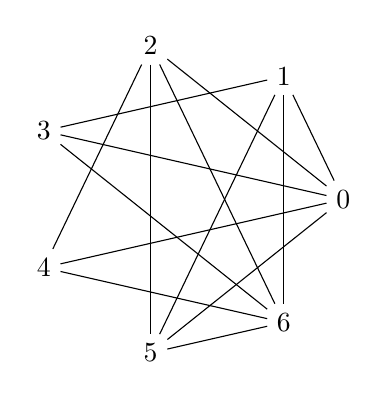
\begin{tikzpicture}
      \draw
        (0.0:2) node (0){0}
        (51.429:2) node (1){1}
        (102.857:2) node (2){2}
        (154.286:2) node (3){3}
        (205.714:2) node (4){4}
        (257.143:2) node (5){5}
        (308.571:2) node (6){6};
      \begin{scope}[-]
        \draw (0) to (1);
        \draw (0) to (2);
        \draw (0) to (3);
        \draw (0) to (4);
        \draw (0) to (5);
        \draw (1) to (3);
        \draw (1) to (5);
        \draw (1) to (6);
        \draw (2) to (4);
        \draw (2) to (5);
        \draw (2) to (6);
        \draw (3) to (6);
        \draw (4) to (6);
        \draw (5) to (6);
      \end{scope}
    \end{tikzpicture}
\end{figure}
\begin{itemize}
\item signature: 111110010110111001011
\item g: Graph with 7 nodes and 14 edges
\item order: 7
\item size: 14
\item max degree: 5
\item degrees: 3,3,4,4,4,5,5
\item is tree: 0
\item is bipartite: 0
\item has bridge: 0
\item is chordal: 0
\item is complete: 0
\item min cycle basis weight: 24
\item min cycle basis size: 8
\item diameter: 2
\item radius: 2
\item is eulerian: 0
\item is planar: 1
\item number of faces: 9
\item is regular: 0
\item p3: 20
\item p4: None
\item property hash: a36904fdd019a7554f2d20da4d0c4368d0a607003ea561c398f376a3086df75c
\end{itemize}
\newpage
\begin{figure}
  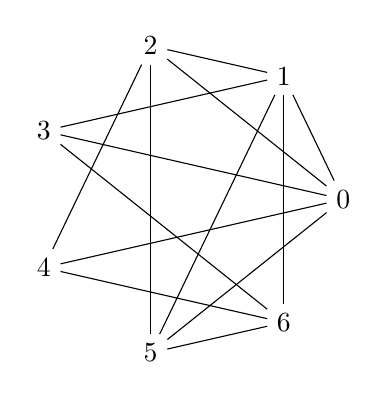
\begin{tikzpicture}
      \draw
        (0.0:2) node (0){0}
        (51.429:2) node (1){1}
        (102.857:2) node (2){2}
        (154.286:2) node (3){3}
        (205.714:2) node (4){4}
        (257.143:2) node (5){5}
        (308.571:2) node (6){6};
      \begin{scope}[-]
        \draw (0) to (1);
        \draw (0) to (2);
        \draw (0) to (3);
        \draw (0) to (4);
        \draw (0) to (5);
        \draw (1) to (2);
        \draw (1) to (3);
        \draw (1) to (5);
        \draw (1) to (6);
        \draw (2) to (4);
        \draw (2) to (5);
        \draw (3) to (6);
        \draw (4) to (6);
        \draw (5) to (6);
      \end{scope}
    \end{tikzpicture}
\end{figure}
\begin{itemize}
\item signature: 111110110110110001011
\item g: Graph with 7 nodes and 14 edges
\item order: 7
\item size: 14
\item max degree: 5
\item degrees: 3,3,4,4,4,5,5
\item is tree: 0
\item is bipartite: 0
\item has bridge: 0
\item is chordal: 0
\item is complete: 0
\item min cycle basis weight: 25
\item min cycle basis size: 8
\item diameter: 2
\item radius: 2
\item is eulerian: 0
\item is planar: 0
\item number of faces: 9
\item is regular: 0
\item p3: 20
\item p4: None
\item property hash: 117f7cef39c383901f7a9d0e9e6576f3679e3b82b47efb3b808b9940b37afabd
\end{itemize}
\newpage
\begin{figure}
  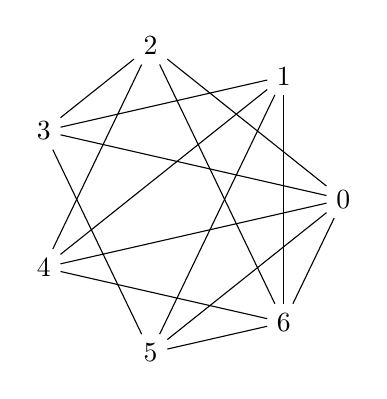
\begin{tikzpicture}
      \draw
        (0.0:2) node (0){0}
        (51.429:2) node (1){1}
        (102.857:2) node (2){2}
        (154.286:2) node (3){3}
        (205.714:2) node (4){4}
        (257.143:2) node (5){5}
        (308.571:2) node (6){6};
      \begin{scope}[-]
        \draw (0) to (2);
        \draw (0) to (3);
        \draw (0) to (4);
        \draw (0) to (5);
        \draw (0) to (6);
        \draw (1) to (3);
        \draw (1) to (4);
        \draw (1) to (5);
        \draw (1) to (6);
        \draw (2) to (3);
        \draw (2) to (4);
        \draw (2) to (6);
        \draw (3) to (5);
        \draw (4) to (6);
        \draw (5) to (6);
      \end{scope}
    \end{tikzpicture}
\end{figure}
\begin{itemize}
\item signature: 011111011111101010011
\item g: Graph with 7 nodes and 15 edges
\item order: 7
\item size: 15
\item max degree: 5
\item degrees: 4,4,4,4,4,5,5
\item is tree: 0
\item is bipartite: 0
\item has bridge: 0
\item is chordal: 0
\item is complete: 0
\item min cycle basis weight: 27
\item min cycle basis size: 9
\item diameter: 2
\item radius: 2
\item is eulerian: 0
\item is planar: 0
\item number of faces: 10
\item is regular: 0
\item p3: 20
\item p4: None
\item property hash: 2b1ab04aef25e599c550233014ad5e06dea62b04c310319fc02ce92fd35be02e
\end{itemize}
\newpage
\begin{figure}
  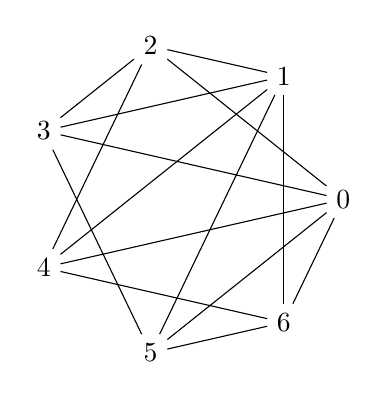
\begin{tikzpicture}
      \draw
        (0.0:2) node (0){0}
        (51.429:2) node (1){1}
        (102.857:2) node (2){2}
        (154.286:2) node (3){3}
        (205.714:2) node (4){4}
        (257.143:2) node (5){5}
        (308.571:2) node (6){6};
      \begin{scope}[-]
        \draw (0) to (2);
        \draw (0) to (3);
        \draw (0) to (4);
        \draw (0) to (5);
        \draw (0) to (6);
        \draw (1) to (2);
        \draw (1) to (3);
        \draw (1) to (4);
        \draw (1) to (5);
        \draw (1) to (6);
        \draw (2) to (3);
        \draw (2) to (4);
        \draw (3) to (5);
        \draw (4) to (6);
        \draw (5) to (6);
      \end{scope}
    \end{tikzpicture}
\end{figure}
\begin{itemize}
\item signature: 011111111111100010011
\item g: Graph with 7 nodes and 15 edges
\item order: 7
\item size: 15
\item max degree: 5
\item degrees: 4,4,4,4,4,5,5
\item is tree: 0
\item is bipartite: 0
\item has bridge: 0
\item is chordal: 0
\item is complete: 0
\item min cycle basis weight: 27
\item min cycle basis size: 9
\item diameter: 2
\item radius: 2
\item is eulerian: 0
\item is planar: 1
\item number of faces: 10
\item is regular: 0
\item p3: 20
\item p4: None
\item property hash: a10e97b496cffa6c4719dbdf15a99d71770b9b1cee9f573ef3ec732deb5c0a6f
\end{itemize}
\newpage
